%%%%%%%%%%%%%%%%%%%%%%%%%%%%%%%%%%%%%%%%%%%%%%%%%%%%%%%%%%%%%%%%%%%%%%
% LaTeX Example: Project Report
%
% Source: http://www.howtotex.com
%
% Feel free to distribute this example, but please keep the referral
% to howtotex.com
% Date: March 2011 
% 
%%%%%%%%%%%%%%%%%%%%%%%%%%%%%%%%%%%%%%%%%%%%%%%%%%%%%%%%%%%%%%%%%%%%%%
% How to use writeLaTeX: 
%
% You edit the source code here on the left, and the preview on the
% right shows you the result within a few seconds.
%
% Bookmark this page and share the URL with your co-authors. They can
% edit at the same time!
%
% You can upload figures, bibliographies, custom classes and
% styles using the files menu.
%
% If you're new to LaTeX, the wikibook is a great place to start:
% http://en.wikibooks.org/wiki/LaTeX
%
%%%%%%%%%%%%%%%%%%%%%%%%%%%%%%%%%%%%%%%%%%%%%%%%%%%%%%%%%%%%%%%%%%%%%%
% Edit the title below to update the display in My Documents
%\title{Project Report}
%
%%% Preamble
\documentclass[paper=a4, fontsize=11.5pt]{scrartcl}
\usepackage[utf8]{inputenc}
\usepackage[T1]{fontenc}
\usepackage{fourier}

\usepackage[english]{babel}                                                         % English language/hyphenation
\usepackage[protrusion=true,expansion=true]{microtype}  
\usepackage{amsmath,amsfonts,amsthm} % Math packages
\usepackage{graphicx}   
\usepackage{import}
\usepackage{grffile}
\usepackage{float}
\usepackage{url}
\usepackage{listings}
\usepackage{arydshln}

%%% Custom sectioning
\usepackage{sectsty}
\allsectionsfont{\normalfont\bfseries}
\usepackage[nottoc,notlot,notlof]{tocbibind}


%%% Custom headers/footers (fancyhdr package)
\usepackage{fancyhdr}
\pagestyle{fancyplain}
\fancyhead{}                                            % No page header
\fancyfoot[L]{}                                         % Empty 
\fancyfoot[C]{}                                         % Empty
\fancyfoot[R]{\thepage}                                 % Pagenumbering
\renewcommand{\headrulewidth}{0pt}          % Remove header underlines
\renewcommand{\footrulewidth}{0pt}              % Remove footer underlines
\setlength{\headheight}{13.6pt}

\newtheorem{defn}{Definition}[section]

%%% Equation and float numbering
\numberwithin{equation}{section}        % Equationnumbering: section.eq#
\numberwithin{figure}{section}          % Figurenumbering: section.fig#
\numberwithin{table}{section}               % Tablenumbering: section.tab#

\setcounter{secnumdepth}{4} % default value for 'report' class is "2"

\usepackage{geometry}

%%% Maketitle metadata
\newcommand{\horrule}[1]{\rule{\linewidth}{#1}}     % Horizontal rule
\usepackage[toc]{glossaries}
%\newglossaryentry{<label>}
%{
  %name=<name>,
  %description={<description>}
  %plural={<termes>}
%}

%\newacronym{<label>}{<abbrv>}{<full>}

%\gls{<label>} %Use the entry
%\gls: singlulier sans majuscule;
%\Gls: singlulier avec majuscule;
%\glspl: pluriel sans majuscule;
%\Glspl: pluriel avec majuscule.


\newglossaryentry{self-dependency}
{
  name=self-dependency,
  description={A dependence from a statement to itself},
  plural=self-dependencies
}


\title{
        %\vspace{-1in}  
        \usefont{OT1}{bch}{b}{n}
        \normalfont \normalsize \textsc{University of Strasbourg} \\ [25pt]
        \horrule{0.5pt} \\[0.4cm]
        \huge High-Level Optimization Driven by Statement Profiling \\
        \horrule{2pt} \\[0.5cm]
}
\author{
        \normalfont                                 \Large
        Thomas Kuntz \\                                \normalsize
        Master RISE \\                                \normalsize
        UFR d'Informatique \\                                \normalsize
        Supervisor : Cédric Bastoul\\
}
\date{}
\makeglossaries
\DeclareUnicodeCharacter{00A0}{ }
%%% Begin document
\begin{document}
%TODO Fill glossary and add link to glossary for used word

\maketitle
\thispagestyle{empty}

\clearpage

\tableofcontents
\clearpage

\section{Presentation of the laboratory and research team}
This intership falls within the research conducted in the ICPS team (Parallel and Scientific
Computing) of the ICube laboratory at the university of Strasbourg, and the CAMUS group
(Compilation for MultiCore Architectures) at Inria, the French Institute for Research
in Computer Science.

\bigskip

ICube is a laboratory created in 2013 and placed under the co-supervision of the Univertisy of
Strasbourg, the CNRS, the ENGEES and the INSA of Strasbourg.
ICube resulted from the consolidation of four former laboratories, namely LSIIT, InESS, IMFS and IPB-LINC,
and aim at bringing together researchers in the fields of engineering science, computer science,
and medical science with imaging as unifying theme.

With around 500 members and under the direction of Michel de Mathelin, ICube is composed of
four different departments, the Computer Science Research Department (D-IR), the
Imaging, Robotics, Remote Sensing and Biomedical Department (D-IRTS), the 
Solid-State Electronics, Systems and Photonics Department (D-ESSP) and the 
Department of Mechanics (D-M).

\bigskip

ICPS (Informatique et Calcul Parallèle et Scientifique)
is one the 5 research team of the Computer Science Research Department of ICube and is
under the supervision of Philippe Clauss.

ICPS research group aspires to contribute to state-of-the-art techniques and
technologies in the field of high performance computing with an area of expertise lying
in the parallelization and optimization of programs.

ICPS hosts as a subset of the team, the INRIA team-project CAMUS.
The ICPS/CAMUS group focuses on providing developers with theoretical and software
tools to develop efficient applications for parallel architectures without sacrificing
productivity.

Parallel systems are now omnipresent, from supercomputers to mobile devices,
and their effective use requires developers to design parallel programs or to rewrite
legacy sequential applications. However, parallel programming is still complex and out
of reach for non experts, at either designing, writing or debugging level.

To address this issue, ICPS/CAMUS is developing source-to-source compiler techniques
for automatic program optimization and parallelization. Using these technologies,
developers can continue to write sequential programs while the mapping to parallel
architecture is computed automatically.

The team has 7 faculty members and a dozen of PhD students,
postdocs or engineers. Its members are deeply involved in European and international
collaborations on scientific projects both with academia and industry.
Its most renowned technical contributions in this field include
the PolyLib library, the code generator CLooG, the dynamic optimizer VMAD or the parallelizer
of binary programs BinPar.


\section{Problematic : High-Level Optimization Driven by Statement Profiling}
Many computation-intensive programs spend a very large amount of their execution
time inside nested loops. Thus, loop nest optimization is one of the major approach used
for program optimisation.

To represent the loop nest, we can use the polyhedral model, a powerful mathematical model
that allows to express loop nest as union of polyhedra and loop optimizations as
transformation of these polyhedra.

The goal is to find the "good" polyhedron transformations to end up with
transformed polyhedra representing loop nest (which doesn't violate dependencies) 
that can be parallelized, vectorized, tiled, etc. with better properties than the original
polyhedron.

The polyhedral model is really good with short and simple codes, but struggles with
large and complex codes.The reason is twofold. First, polyhedral techniques exhibit
a very high worst-case complexity which hampers its applicability to large codes.
Second, contradicting optimization objectives may result in suboptimal global
decisions


We would like to address these issues by proposing a new technique : before any
high-level optimizations are used on the source code, a first pass is applied (our pass),
aggregating "near behaving" statements together using their profile.
By doing that, we hope to ease the work of the high-level optimizer by "reducing" the size
of large and complex code, and prevent it from separating statements that should
not be separated (for example if they share a lot of data reuse).

"Near behaving" statements describe statements that have similar properties,
like data reuse/locality, parallelism, vectorization etc. that constitute their profile.

To achieve that, we first need to learn about the different properties. Then in a second
time, we need to find a way to measure/quantify them statement-wise. Then, in a third
time we need to find a way to compute, to \textit{"rate"}, the similarity of the different
properties between two statement. Then in the end, we will try to find smart algorithms
that produce the best aggregated set of statements, based on the rate computed.

%{The reasons behind the choice of this internship}
\section{The reasons behind the choice of this internship}
The first reason why I've asked and chosen this internship was that I wanted to see
if I was capable enough, if I had what it takes to work in research, or if it was more than I could
chew.

The second was that I also wanted to put myself to the test and see if I really 
wanted to try to do a PhD or not : I wanted to know if I could be as interested in being
a researcher as I was interested in being a college teacher in Computer Science
(because it's hard in France to be the second without being the first one).

In other words,
I was expecting this internship to be a little bit like a trial by fire that would help me
take a decision for my professional future.

\bigskip

In addition to these reasons, which were more intimate and personal than practical, the
other reasons behind my choice were :
\begin{itemize}
    \item[] I wanted to learn more about optimization methods, both high and low level methods,
        to know more about what can be done when trying to optimize a code by hand.
    \item[] I was also expecting to learn some valuable skills :
        \begin{itemize}
            \item To be able to do a literature review about the state of the art techniques of
                a subject (here : code optimization techniques).
            \item To become more familiar with reading, analyzing and summarizing scientific papers.
            \item To become more familiar with benchmarking, performance analysis and
                graphical representation of data.
            \item To become more familiar with the use of external libraries, project
                management and become more fluent in C and Python.
        \end{itemize}
\end{itemize}

\bigskip

Those were all the reasons that motivated my choice.


\section{General Informations}
%\section*{General Informations}
%\addtocontents{toc}{\protect\contentsline{section}{General Informations}{}}

    In this report, several things should be noted :
    \begin{itemize}
        \item Arrays used in code example are always in Row-major layout.
        \item Code example are either in C or pseudo-code.
    \end{itemize}

\section{polyhedral model}
The first thing I had to do during this internship was to learn everything about the polyhedral
model, because it was intended to use this model to abstract the program we are trying
to optimize. I explain in this section what I've learned about the polyhedral model during
this internship.

\bigskip

The polyhedral model is (as explained in the thesis~\cite{Bas'12}) a mathematical
model that allows to represent program parts as union of polyhedra and affine sets.
Program parts that can fit the model are called \textit{static control parts} or
\textit{SCoPs} for short. Scops are generally loop-based, and need to have affine loop bounds,
and conditions/array subscripts that fit the polyhedral model (they need to be affine).

The polyhedral model consist of three mathematical objects based on unions of relations :
\begin{itemize}
    \item The \textit{Iteration Domain}, that provide the set of all the iteration scanned
        %parcouru
        by a specific statement, using affine constraints. It's these affine constraints 
        that can be seen as a $\mathbb{Z}$-polyhedron.
    \item The \textit{Scattering Relations} (or \textit{Scheduling Relations},
        or even \textit{Mapping Relations}), that give us the ordering in which
        all the statement instances will be executed.
    \item The \textit{Access Relations} that models read/write accesses made by
        the different arrays and variables or the scop.
\end{itemize}

    \subsection{Iteration Domain}
        To understand the \textit{Iteration Domain}, it's necessary to first understand
        what a \textit{statement instance} is. A statement instance is one particular
        execution of a statement. When a statement is located inside a loop nest, 
        it can be associated with the value of the all the outer-loop counters
        (called \textit{iterators}) of the statement.\\
        The Iteration Domain will be the set of the iterators of all the statement
        instances.

        Because the outer loop bound can be affine or parameterized, it is generally impossible to
        know their actual value at compilation time. Even if we knew the value of the
        bounds, the number of iterators could be too enormous to count and list them all into sets.
        That's why the sets are expressed as a system of affine constraints.
        These affine constraints define a $\mathbb{Z}$-polyhedron, hence the name of the model.
        The relation used to represent the Iteration Domain is :
        \begin{center}
            $ \mathcal{D}_S(\vec{p}) = \left\{() \to \vec{\imath_S} \in \mathbb{Z}^{\dim(\vec{\imath_S})}
            \middle|
            \left[D_S\right]\begin{pmatrix}\vec{\imath} \\ \vec{p} \\ 1\end{pmatrix}
            \geq \vec{0}
            \right\}$
        \end{center}
        where $\vec{p}$ is the parameter vector, $\vec{\imath_S}$ the $\dim(\vec{\imath_S})$-dimensional iteration vector and
        $D_S \in \mathbb{Z}^{m_{\mathcal{D}_S} \times (\dim(\vec{\imath})+\dim(\vec{p})+1)}$
        is an integer matrix where $m_{\mathcal{D}_S}$ is the number of constraints.
        \\

\begin{lstlisting}[frame=single, language=C, caption={Simple code for polyhedral model example}, label={lst:polyhedral_example}]
        for(i=0 ; i<2*N - 1 ; i++)
S1:         A[i] = 42;
        for(i=0 ; i<N ; i++)
            for(j=0 ; j<N ; j++)
S2:             B[i][j] += 42;
\end{lstlisting}
        
        For example, in Listing~\ref{lst:polyhedral_example}, we have for
        S1 and S2 the iteration domain :
        \begin{itemize}
            \item[]$ \mathcal{D}_{S1}(N) = \left\{() \to \begin{bmatrix}i\end{bmatrix} \in \mathbb{Z} \middle|
            \left[\begin{array}{c:c:c}
                    1 & 0 & 0 \\
                    -1 & 2 & -2
            \end{array}\right]
            \left(\begin{array}{c}
                    i \\ \hdashline
                    N \\ \hdashline
                    1 
            \end{array}\right)
            \geq \vec{0}
            \right\} $,
        
            \item[]$ \mathcal{D}_{S2}(N) = \left\{() \to \begin{bmatrix}i\end{bmatrix} \in \mathbb{Z} \middle|
            \left[\begin{array}{c:c:c:c}
                    1 & 0 & 0 & 0\\
                    -1 & 0 & 1 & -1\\
                    0 & 1 & 0 & 0\\
                    0 & -1 & 1 & -1
            \end{array}\right]
            \left(\begin{array}{c}
                    i \\
                    j \\ \hdashline
                    N \\ \hdashline
                    1 
            \end{array}\right)
            \geq \vec{0}
            \right\} $.
        \end{itemize}

        In the case of \textit{if-then-else} enclosed statements, the iteration domain
        for the statement will be an union of disjoint polyhedron, each representing a part
        of the \textit{if-then-else} condition.

    \subsection{Scattering Relations}
        Defining the domain of iteration is great, but it doesn't give us any information
        on the order in which will be executed each statement instance.

        There are different types of ordering relations :
        \begin{description}
            \item[Scheduling] is about ordering the statement instances in time by
                giving them a logical date vector indicating when each will be executed.
                The data vector is generally read in \textit{lexicographical} order, for example
                $(1,2,3)$ is executed before $(1,2,4)$ but after $(1,1,4)$.
            \item[Allocation] or \textbf{placement} is about ordering statement instances
                in space by assigning to each statement instances a logical stamp
                indicating the processor number in which it will be executed.
                Statement instances not sharing the same logical stamp can be
                executed in parallel in different processors.
        \end{description}

        It is possible to express each ordering relations separately,
        but it is also possible to aggregate them together : the result would be
        a relation between the iterators set and a set of ordering vectors which
        would have some dimensions allocated to time ordering (scheduling) and
        some other to space ordering (allocation).

        For a statement $S$, the scattering relation can be written as follow :
        \begin{center}
            $\theta_S(\vec{p}) = \left\{\vec{\imath_S} \to \vec{t_S} \in \mathbb{Z}^{\dim(\vec{\imath_S})}\times\mathbb{Z}^{\dim(\vec{t_S})}
            \middle|
            \left[T_S\right]\begin{pmatrix}\vec{t_S}\\ \vec{\imath} \\ \vec{p} \\ 1\end{pmatrix}
            \geq \vec{0}
            \right\}$,
        \end{center}
        where $\vec{p}$ is the parameter vector, $\vec{\imath_S}$ the $\dim(\vec{\imath_S})$-dimensional iteration vector
        and $T_S \in \mathbb{Z}^{m_{\theta_S}\times(\dim(\vec{\imath_S})+\dim(\vec{t_S})+\dim(\vec{p})+1)}$
        is an integer matrix where $m_{\theta_S}$ is the number of constraints.

        For example, for Listing~\ref{lst:polyhedral_example}, we have for S1 and S2
        statement the following original scattering :
        \begin{itemize}
            \item[]
                $\theta_{S1}(N) = \left\{(i) \to \begin{pmatrix}t^{1}_{S1}\\t^{2}_{S1}\\t^{3}_{S1}\end{pmatrix} \in
                    \mathbb{Z}\times\mathbb{Z}^{3}
                    \middle|
                    \left[\begin{array}{ccc:c:c:c}
                            -1 & 0 & 0 & 0 & 0 & 0 \\
                            0 & -1 & 0 & 1 & 0 & 0 \\ 
                            0 & 0 & -1 & 0 & 0 & 0
                    \end{array}\right]
                    \left(\begin{array}{c}
                        t^{1}_{S1} \\
                        t^{2}_{S1} \\
                        t^{3}_{S1} \\ \hdashline
                        i \\ \hdashline
                        N \\ \hdashline
                        1
                    \end{array}\right)
                    = \vec{0}
                    \right\}$,\\
                    which can be simplified to $\theta_{S1}(N)(i)=\begin{pmatrix}0\\i\\0\end{pmatrix}$.
            \item[]
                $\theta_{S2}(N) = \left\{(i) \to \begin{pmatrix}t^{1}_{S2}\\t^{2}_{S2}\\t^{3}_{S2}\\t^{4}_{S2}\\t^{5}_{S2}\end{pmatrix} \in
                    \mathbb{Z}\times\mathbb{Z}^{3}
                    \middle|
                    \left[\begin{array}{ccccc:cc:c:c}
                            -1 & 0 & 0 & 0 & 0 & 0 & 0 & 0 & 1\\
                            0 & -1 & 0 & 0 & 0 & 1 & 0 & 0 & 0\\ 
                            0 & 0 & -1 & 0 & 0 & 0 & 0 & 0 & 0\\
                            0 & 0 & 0 & -1 & 0 & 0 & 1 & 0 & 0\\ 
                            0 & 0 & 0 & 0 & -1 & 0 & 0 & 0 & 0
                    \end{array}\right]
                    \left(\begin{array}{c}
                        t^{1}_{S2} \\
                        t^{2}_{S2} \\
                        t^{3}_{S2} \\
                        t^{4}_{S2} \\
                        t^{5}_{S2} \\ \hdashline
                        i \\ \hdashline
                        N \\ \hdashline
                        1
                    \end{array}\right)
                    = \vec{0}
                    \right\}$,\\
                    which can be simplified to $\theta_{S2}(N)\begin{pmatrix}i\\j\end{pmatrix}=\begin{pmatrix}1\\i\\0\\j\\0\end{pmatrix}$.
        \end{itemize}
        The first dimension for S1 is 0 and for S2 is 1 : it is to ensure that S2
        is always executed after S1. This dimension is also an example of \textit{Scheduling} dimension.
        In our example, it doesn't matter because S1 and S2 don't have any data dependence
        whatsoever, and they could be run in parallel without problem, but for the sake
        of the example, we've imposed that S1 is executed before S2.

    \subsection{Access Relations}
        The \textit{Access Relations} model the different memory accesses made 
        in a statement. It maps the statement instances to memory locations
        for every array reference of a statement. Non-array references like simple variable
        can be seen as 0-dimensional array.

        The access relation can be written in the general form :
        \begin{center}
            $\mathcal{A}_{S,r}(\vec{p}) = 
            \left\{
                \vec{\imath_S} \to \vec{a}_{S,r} \in \mathbb{Z}^{\dim(\vec{\imath_S})}\times\mathbb{Z}^{\dim(\vec{a}_{S,r})}
                \middle|
                \left[A_{S,r}\right]\left(\begin{array}{c}\vec{a}_{S,r}\\\vec{\imath_S}\\\vec{p}\\1\end{array}\right)
                \geq \vec{0}
            \right\}$
        \end{center}
        where 
        \begin{itemize}
            \item $\vec{p}$ is the parameter vector.
            \item $r$ is the number of the reference in the statement (every references are
                numbered, from left to right generally).
            \item $\vec{\imath_S}$ is the $\dim(\vec{\imath_S})$-dimensional iteration vector
            \item $T_S \in \mathbb{Z}^{m_{\theta_S}\times(\dim(\vec{\imath_S})+\dim(\vec{t_S})+\dim(\vec{p})+1)}$
                is an integer matrix where $m_{\theta_S}$ is the number of constraints.
        \end{itemize}

        The read or write nature of the memory access is not expressed in this form,
        and needs to be given alongside the model (for example, to compute data dependencies).

        %TODO Expliquer les outputs dimensions (si il y en as dans le modèle théorique).

        For example, for Listing~\ref{lst:polyhedral_example}, we have for S1 and S2 the
        access relation :
        \begin{itemize}
            \item[]
                $
                \mathcal{A}_{S1,1}(N) = 
                \left\{
                \begin{pmatrix}i\end{pmatrix} \to \left(a_{S1,1}\right) \in \mathbb{Z}\times\mathbb{Z}
                    \middle|
                    \left[\begin{array}{c:c:c:c}-1 & 1 & 0 & 0 \end{array}\right]
                    \left(\begin{array}{c}a_{S1,1}\\\hdashline i\\\hdashline N\\\hdashline 1\end{array}\right)
                    = \vec{0}
                \right\}
                $
            
            \item[]
                $
                \mathcal{A}_{S2,1}(N) = 
                \left\{
                \begin{pmatrix}i\end{pmatrix} \to \left(a_{S2,1}\right) \in \mathbb{Z}\times\mathbb{Z}
                    \middle|
                    \left[\begin{array}{c:c:c:c:c}-1 & 1 & 0 & 0 & 0 \\
                                                  -1 & 0 & 1 & 0 & 0 \end{array}\right]
                    \left(\begin{array}{c}a_{S2,1}\\\hdashline i\\\hdashline j\\\hdashline N\\\hdashline 1\end{array}\right)
                    = \vec{0}
                \right\}
                $
        \end{itemize}

        Because S1 and S2 only have one reference, there's only one access relation for
        each of them.

    \subsection{Dependence Relations}
    \label{sec:dependence_relations}
        Data Dependencies are necessarily considered, when, for example, we have to identify if a statement
        can be parallelized or vectorized (simdized). They are also needed when we try to
        transform the scattering of a statement : doing that could violate dependencies between
        some statements, and the Dependence Relations (with Violation Relations) can be used to detect such
        violations.

        Fortunately, Data Dependency can be easily represented in the polyhedral model as
        \textbf{Dependence Relation}.

        A Dependence Relation represent the fact that some ordered statement iterations
        access the same memory location. The general form of the Dependence Relation of
        a dependency between a \textit{source} statement $S$ and a \textit{target}
        statement $T$ at a depth $d$ is the following (explained after) :

        \begin{center}
        \scalebox{0.85}{
            ${
            \delta_{S,r_S \xrightarrow{d} T,r_T}(\vec{p}) =
                \left\{
                \begin{pmatrix}\vec{\imath}_S \\ \vec{a}_{S,r_S} \end{pmatrix}
                \to
                \begin{pmatrix}\vec{\imath}_T \\ \vec{a}_{T,r_T} \end{pmatrix}
            \middle|
                \left[\begin{array}{c:c|c:c|c:c}
                    D^{\vec{\imath}_S}_{S} & 0 & 0 & 0 & D^{\vec{p}_S}_{S} & D^{c}_{S} \\ \hdashline
                    0 & 0 & D^{\vec{\imath}_T}_{T} & 0 & D^{\vec{p}_T}_{T} & D^{c}_{T} \\ \hline
                    A^{\vec{\imath}_S}_{S,r_S} & A^{\vec{a}_{S,r_S}}_{S,r_S} & 0 & 0 & D^{\vec{p}}_{S,r_S} & D^{c}_{S,r_S} \\ \hdashline
                    0 & 0 & A^{\vec{\imath}_T}_{T,r_T} & A^{\vec{a}_{T,r_T}}_{T,r_T} & D^{\vec{p}}_{T,r_T} & D^{c}_{T,r_T} \\ \hdashline
                    0 & I & 0 & -I & 0 & 0 \\ \hline
                    I^{1..d-1,\bullet} & 0 & -I^{1..d-1,\bullet} & 0 & 0 & 0 \\ \hdashline
                        I^{d,\bullet} & 0 & -I^{d,\bullet} & 0 & 0 & 0\text{ or }-1 \\
                \end{array}\right]
                %\quad
                \begin{pmatrix}{c}
                    \vec{\imath}_S \\ \hdashline
                    \vec{a}_{S,r_S} \\ \hline
                    \vec{\imath}_T \\ \hdashline
                    \vec{a}_{T,r_T} \\ \hline
                    \vec{p} \\ \hdashline
                    1 \\
                \end{pmatrix}
                \quad
                \begin{matrix}
                    \geq \\ \hdashline
                    \geq \\ \hline
                    \geq \\ \hdashline
                    \geq \\ \hdashline
                    = \\ \hline
                    = \\ \hdashline
                    \geq \\
                \end{matrix}
                \vec{0}
                \right\}
            }$
        }
        \end{center}
        If, for the statement $S$ and $T$ and with the depth $d$, this relation is not empty
        (meaning that with all these constraints, there is still at least a point in the set
        this relation represents) then there is a dependency between $S$ and $T$.
        
        This matrix seems complicated at first but we are just piling up more and more constraints
        on a linear system. Theses constraints correspond to three sub-relations :
        \begin{itemize}
            \item First, there is the \textbf{Existence Condition} of the instances.
                It corresponds to the lines 1-2 of the matrix.

                The \textit{Existence Conition} determines, like in the \textit{Domain Relation},
                the set of possible iterations for the 2 statements (a dependency couldn't
                possibly exist between out-of-\textit{Domain} iterations).

                It's just the \textit{Domain Matrix} of the 2 statements split vertically
                in 3 and placed correctly in the \textit{Dependence Matrix}.
            \item Second, there is the \textbf{Conflit Condition} of the memory location.
                It corresponds to the lines 3-4-5 of the matrix.

                The \textit{Conflict Condition} determines the equality of the 2 different 
                memory accesses causing the dependency : if there is a dependency,
                it means that for some iterations, these 2 memory accesses
                access the same memory location, so it means that for some iterations,
                the 2 memory accesses are equal.

                To represent that, we add to the system the \textit{Access Matrix} of the 2 memory accesses
                causing the dependency and then a series of constraints
                binding the two accesses into equality (Identity matrix for the first
                \textit{Access Matrix} , and a negative Identity matrix for the second).
            \item Third, there is the \textbf{Causality Condition} of the instances.
                It corresponds to the line 6-7 of the matrix.

                The \textit{Causality Condition} makes sure that the iterations of the
                \textit{source} statement are executed before the ones of the \textit{target} statements
                involved in the dependency.

                We define what is called the \textit{dependence depth} $d$. There are
                as many possible $d$ as there are of loops in common between the statements $S$ and $T$.
                If for a value of $d$, the linear system represented by the \textit{Dependence Matrix}
                has a solution, it means that the loop of depth $d$ carry the dependency.
                If multiple values of $d$ produce solutions to the linear system (so there
                is multiple \textit{Dependence Relation} for the same statements and
                memory locations/accesses), it means that multiple loops carry the dependency.

                To add the notion of \textit{Causality} we add to the system a series of
                constraints binding the corresponding \textit{source} and \textit{target}
                iterators of the loops having a depth $d'$ lighter than $d$
                (with a Identity and negative Identity matrix).
                For the \textit{source} and \textit{target} iterator of the loop having
                the depth $d$, instead of an equality, we bind them with an inequality :
                the \textit{source} iterator lighter than or equal to ($\leq$) the \textit{target} iterator.

                It's also possible to force a strict inequality ($<$) by setting the cell
                in the last line and column of the matrix to $-1$, instead of $0$.
        \end{itemize}

        \medskip
        
        To illustrate the \textit{Dependence Matrix}, we would like to introduce a piece of code :
\begin{lstlisting}[frame=single, language=C, caption={Simple code for Dependence Relation example}, label={lst:dependence_example}]
for(i=1 ; i<N ; i++)
{
        A[i] = 42;
        B[i] = A[i-1]
}
\end{lstlisting}
        
        For example, in the Listing~\ref{lst:dependence_example}, we can see a Read-after-Write
        dependency : when $(i=1)$ we write in $A[1]$, and when $(i=2)$ (the next iteration)
        we read in $A[1]$ (and write in $A[2]$ but the location is different so that's not important here).

        For this dependency, we would have the following \textit{Dependence Matrix} :
\begin{center}
$
        \begin{array}{c:c|c:c|c:c}
        i &    [0] & i' &   [0]' &  N &  1 \\ \hline \hline
        1 &    0 &   0 &    0 &   0 &  -1 \\
        -1 &    0 &   0 &    0 &   1 &  -1 \\
        0 &    0 &   0 &    0 &   1 &  -2 \\ \hdashline
        0 &    0 &   1 &    0 &   0 &  -1 \\
        0 &    0 &  -1 &    0 &   1 &  -1 \\
        0 &    0 &   0 &    0 &   1 &  -2 \\
        1 &   -1 &   0 &    0 &   0 &   0 \\ \hline
        0 &    0 &  -1 &    1 &   0 &   1 \\ \hdashline
        0 &   -1 &   0 &    1 &   0 &   0 \\ \hline
        -1 &    0 &   1 &    0 &   0 &   0 \\
        \end{array}
        \qquad
        \begin{matrix}
                \\ \hline \hline
        {i-1 >= 0} \\
        {-i+N-1 >= 0} \\
        {N-2 >= 0} \\ \hdashline
        {i'-1 >= 0} \\
        {-i'+N-1 >= 0} \\
        {N-2 >= 0}  \\
        {i-[0] == 0}\\ \hline
        {-i'+[0]'+1 == 0} \\ \hdashline
        {[0] - [0]' == 0}  \\ \hline
        {-i+i' >= 0} \\
        \end{matrix}
$
\end{center}
    with :
    \begin{itemize}
        \item $[0]$ and $[0]'$ the first (and only) dimension of respectively \verb'A[i]' and
            \verb'A[i-1]'.
        \item $i$ and $i'$ the iterators of respectively \verb'A[i]' and \verb'A[i-1]'
            (here $i$ and $i'$ are the same, but iterators are always considered different).
        \item A dependence depth $d = 1$.
    \end{itemize}
    
    If we pass this matrix in any linear solving software (like PIP~\cite{Fea88}) and try to solve it,
    we would get solutions, meaning that the dependency exists.

    \bigskip

    That's really one of the most powerful side of the polyhedral model, its ability to
    compute the different dependencies by building linear systems : if there is a solution,
    there is a dependency, and if not, there is no dependency. It's powerful because
    the techniques to build and solve linear systems are known and mastered, so the basis
    of the model is really strong and stable. 


    \subsection{OpenScop Framework}
        OpenScop~\cite{openscop} is an open specification that defines a file format
        and a set of data structures to represent a static control part (SCoP).

        OpenScop format is intended to be a stable bridge between polyhedral tools
        and optimizers allowing interchangeable tools and flexible toolchains.

        A library named \textit{osl} is provided to read/write OpenScop files
        and manipulate the different data structures the specification defines.
        The file format as well as the library has been designed to accept extensions.

        Substrate, the tool I have written during this internship to perform our analysis
        and optimization pass uses \textit{osl} OpenScop as input and output format.

\section{Statement Profiling}
In this section we will present and explain the different properties a statement can exhibit
that can characterize similarity. We will then present and discuss the model we chose to model
those properties.\\
This list is composed of the properties we had time to study, select and implement,
and it is of course not exhaustive : other profile types need to be considered in the future.
\label{sec:statement_profiling}
    \subsection{Data Reuse/Locality}
        In this section, we will explain the basics behind data reuse/locality. We will then
        talk about the different metrics and methods found in the literature used to evaluate
        and quantifying data reuse, why they where selected/kept in mind or not for the \textit{Reuse Profile}.
        And finally we will discuss the final model we have chosen for the \textit{Reuse Profile}.

        \subsubsection{Difference between Reuse and Locality}
            It's important to differentiate \textit{reuse} from \textit{locality}.
            We say that there is \textit{reuse} for a data when this data is
            accessed multiple times during the execution of a loop nest, during
            the same iteration or not. It can be from different references or different statements.
            
            When there is reuse, it's possible (but not guaranteed) to have
            \textit{locality}. We say that there is \textit{locality} when the
            reused data remains in the memory hierarchy level targeted 
            (eg : the CPU cache in our case) between 2 reuses.
            For that to be the case, the amount of other data accessed between the
            2 reuses must not exceed the cache size, or else the reused data will be
            evicted from the cache, causing a cache miss and forcing the cache
            to fetch the data from the RAM (and RAM have higher latency compared to CPU cache).


            Thus, we can say that the \textit{reuse} is linked to the way indexing
            functions/subscripts (for array references) are written, whereas \textit{locality} is
            inherent to the iterations order.

\medskip

        \subsubsection{Types of Reuse}
            
\begin{lstlisting}[frame=single, language=C, caption=Reuse example, label={lst:reuse_example}]
for(i=0; i<N ; i++)
    for(j=0; j<N ; j++)
    {
        A[i][j] = B[i] + B[i+1];
        C[i][j] = B[i+2] * 2;
    }
\end{lstlisting}

            \paragraph{Self-Temporal}
                Self-Temporal reuse occurs when the same reference accesss the same
                data location.
                
                For example, in Listing \ref{lst:reuse_example}, the reference \verb'B[i]' carries Self-Temporal
                reuse :\verb'B[0]',\verb'B[1]',\verb'B[2]' ... \verb'B[N-1]' are accessed
                \textit{j} times by the same reference \verb'B[i]'.
                And for the same reason, \verb'B[i+1]' and \verb'B[i+2]' also carry Self-Temporal reuse.

            \paragraph{Self-Spatial}
                Self-Spatial reuse occurs when the same reference accesses the same
                line in an array (when in row-major). Especially, the space between
                two accessed data locations should not be greater than a cache line size,
                or else there won't be any spatial locality.

                For example, in Listing \ref{lst:reuse_example}, the reference \verb'A[i][j]' carries
                Self-Spatial reuse.

                Self-Temporal reuse can be considered as a special case of
                Self-Spatial reuse : accessing the same data location means that
                the same array line is also accessed.
            \paragraph{Group-Temporal}
                Group-Temporal reuse occurs when different references access the same
                data location. It can occur inside a same statement or across different
                statements.

                For example, in Listing \ref{lst:reuse_example}, the references
                \verb'B[i]', \verb'B[i+1]' and \verb'B[i+2]' carry Group-Temporal :
                the data accessed by \verb'B[i+2]' when $i=M$ will be accessed by
                \verb'B[i+1]' when $i=M+1$ and by \verb'B[i]' when $i=M+2$.

            \paragraph{Group-Spatial}
                Group-Spatial reuse occurs when different references access the same
                line in an array (when in row-major). Again, the space between
                two accessed data locations should not be greater than a cache line size,
                or else there won't be any spatial locality.
                
                For example, in Listing \ref{lst:reuse_example}, the references
                \verb'B[i]', \verb'B[i+1]' and \verb'B[i+2]' carry Group-Spatial :
                they all access to different data location, but on the same line.\\
                \\

                So as we can see, a single reference can carry multiple type of reuse.
                A statement being generally composed of multiple references, it 
                can be hard to automatically favor some statements instead of others.
        \subsubsection{Reuse Vector Space}
        \label{sec:wolf_91}
            The notion of Reuse Vector Space comes from Wolf et. al.\cite{Wolf'91} and describes
            the vector subspace of the Iteration vector space where the reuse of
            a reference can effectively induce locality.
            There are as many reuse vector space as there are types of reuse.

\begin{lstlisting}[frame=single, language=C, caption=Simple example, label={lst:simple_example}]
for(i=0; i<N ; i++)
    for(j=0; j<N ; j++)
    {
        f(A[i], A[j]);
    }
\end{lstlisting}

            For example, in Listing \ref{lst:simple_example}, with the Iteration
            space being spanned by $\{(1,0),(0,1)\}$, the self-spatial reuse vector space of
            \verb'A[i]' is $\{(1,0)\}$ (ie the {\it i} loop), and \verb'A[j]''s is $\{(0,1)\}$
            (ie the {\it j} loop).

            Wolf et. al. uses the concept of uniformly generated references proposed
            by Gannon et. al.\cite{Gannon:1988:SCL:50454.50460} for estimating reference
            windows :
            \begin{defn}
            \label{sec:uniformly_generated}
                Let $n$ be the depth of a loop nest, and $d$ be the dimensionality of
                an array $A$. Two references $A[\vec{a}(\vec{\imath})]$ and
                $B[\vec{b}(\vec{\imath})]$, where $\vec{a}$ and $\vec{b}$ are indexing
                functions $Z^{n} \rightarrow Z^{d}$, are called \textbf{uniformly generated} if :
                \begin{center}
                    $\vec{a}(\vec{\imath}) = H\vec{\imath}+\vec{c}_a$ and $\vec{b}(\vec{\imath}) = H\vec{\imath}+\vec{c}_b$
                \end{center}
                where $H$ is a linear transformation and $\vec{c}_a$ and $\vec{c}_b$ are constant vectors.
            \end{defn}
            
            We can partition references into equivalence classes, called \textit{uniformly generated sets},
            when the references operate on the same array, and have the same $H$.
            We can see $H$ as a part of one of the access functions (in the polyhedral model representation) of this statement :
            it's the access function matrix without the part handling the constant vector.

            For example in Listing \ref{lst:reuse_example}, $B[i]$,$B[i+1]$ and $B[i+2]$ can each be written as
            \begin{center}
                $
                \begin{bmatrix}
                    1 & 0
                \end{bmatrix}
                \begin{bmatrix}
                    i\\
                    j
                \end{bmatrix}
                +
                \begin{bmatrix}
                    0
                \end{bmatrix}
                $,\\
                $
                \begin{bmatrix}
                    1 & 0
                \end{bmatrix}
                \begin{bmatrix}
                    i\\
                    j
                \end{bmatrix}
                +
                \begin{bmatrix}
                    1
                \end{bmatrix}
                $,\\
                $
                \begin{bmatrix}
                    1 & 0
                \end{bmatrix}
                \begin{bmatrix}
                    i\\
                    j
                \end{bmatrix}
                +
                \begin{bmatrix}
                    2
                \end{bmatrix}
                $.
            \end{center}
            As we can see, all these references share the same $H=\begin{bmatrix}1 & 0\end{bmatrix}$,
            so they all belong to the same class.\\
            Of course, $B[i]$,$B[i+1]$ and $B[i+2]$ belong to different statements, and in
            our pass, a uniformly generated set would be created for each statement.

            The problem with that method, is that it would put the references
            $C[i][j],C[i][j+1],C[i-1][j]$ in the same class : they all share the
            same $H$, but they don't have the same reuse space at all.
            For example : $C[i][j],C[i-1][j]$ exhibit group-spatial reuse in the $i$ dimension,
            whereas $C[i][j],C[i][j+1]$ exhibit group-spatial reuse in the $j$ dimension. So they
            should not be grouped together in the same class.
            \medskip

            So the definition of the \textit{uniformly generated set} is not restrictive enough,
            but we will use it as a base for our model.



        \subsubsection{The Simple Algorithm}
            The \textit{Simple Algorithm}~\cite{Kennedy94maximizingloop} is an
            optimization algorithm that improves data locality via Loop Fusion.
            The idea is to fuse vertices of a directed graph when those vertices
            are connected by non-fusion-preventing arcs.
            In this graph, the vertices represent the different loop nests of a program part,
            and the arcs represent data dependencies between statements of different loop nests.

            If the dependency is fusion-preventing~\cite{Bacon:1994:CTH:197405.197406} or if the loop headers are incompatible,
            the arc representing the dependency will be marked fusion-preventing.

            The algorithm is a modification of the greedy algorithm that partitions
            the nodes of the graph without sequentializing a parallel node/loop, and
            is the following (directly taken from~\cite{Kennedy94maximizingloop}:
            \medskip

            ``  In the greedy partition graph, if there exists two partitions $g_1$
                and $g_2$ with a directed edge $(g_1,g_2)$, then no node in $g_2$
                may be legally placed in $g_1$ or the greedy algorithm would have put it
                there. However, it may be safe and profitable to move nodes in $g_1$
                down into $g_2$.

                We determine if it is safe and profitable to move $n \in g_l$ down
                into another partition $g_h$ as follows.
                \begin{description}
                        %TODO check iff
                    \item [Safety.] A node $n \in g_l$ may move to $g_h$ \textit{iff} it
                        has no successors in $g_l$ and there is no fusion-preventing
                        edge $(n,r)$ such that $r \in g_h$ or $r \in g_k$ where
                        $g_k$ must precede $g_h$.
                    \item [Profitability.] Computes a sum of edges $(m,n), m \in g_l$
                        and a sum for each $g_h$ of edges $(n,p)$ such that $p \in g_h$
                        and $n$ may be safely moved into $g_h$. Pick the partition
                        $g$ with the biggest sum. If $g \neq g_l$, move $n$ down into $g$.''
                \end{description}
            \bigskip
            
            This algorithm doesn't give us any metric or way to evaluate a statement
            reuse, so it doesn't help use for the reuse evaluation side, but the idea
            of a dependency graph based greedy algorithm is interesting : with statement
            instead of loop nest being the nodes, this kind of greedy algorithm 
            could fuse statements that are inside different loop nests in the SCoP.
            Meaning we would also need to redefine the \textbf{Safety} and \textbf{Profitability}
            notions of the algorithm.

        \subsubsection{Data and Loop Transformations Algorithm}
            An algorithm that transforms a loop nest to improve cache locality
            by a combination of loop and data transformations is presented in~\cite{Kandemir99improvingcache}.

            There's not much to say about it. The goal of the algorithm is to
            compute a transformation matrix and array layout (and the explanation is a little
            vague), so it isn't applicable in our case and it doesn't give us any metric or way to evaluate the reuse.
        
        \subsubsection{LoopCost Algorithms}
            The LoopCost algorithm~\cite{McKinley:1996:IDL:233561.233564} provides
            us with a cost model that allow to help us chose the right loop transformation like
            loop permutation, loop reversal, loop fusion, loop distribution,
            by comparing the cost with and without the transformation.
            
            The LoopCost algorithm works like this : 
            Each loop $l$ in a loop nest is considered as a candidate for the innermost
            position in the nest. For each loop $l$, LoopCost computes and sums the number
            of cache line accesses by a group of references (the groups are formed
            using the RefGroup algorithm) when $l$ is placed as the innermost loop.

            As a result, we have a cost for each loop when they are considered as innermost.
            This cost enables the possibility to compare a loop nest with hard numbers 
            before and after some loop transformations, which allows us to discard
            or apply the transformations if the new cost is worse or better than the
            original cost.
            \bigskip

            Because the LoopCost is loop transformation oriented and because it doesn't
            use the number of references in a reference group for the computation
            of the cost, it is not really applicable to our situation.

            Regarding the RefGroup algorithm that partitions the array references
            in group, the criteria used are like the ones for \textit{uniformly generated set}
            but a little more restrictive, and we don't need more restrictive, so we won't
            be able to use them.
            
            
        \subsubsection{Automatic Polyhedral Parallelization and Locality Optimization Algorithm}
        \label{sec:auto_poly_paral}
            Let $S_i$ and $S_j$ two statement of a program with a data dependency $e$
            from $S_i$ to $S_j$.\\
            Let $\vec{s}$ and $\vec{t}$ the iterators of respectively $S_i$ and $S_j$.\\
            Let $\theta_{S_i}$ and $\theta_{S_j}$ the scattering function of respectively $S_i$
            and $S_j$.\\
            Consider the following affine $\delta_e$ :
            \begin{center}
                $\delta_e\left(\vec{s},\vec{t}\right) = \theta_{S_j}\left(\vec{t}\right) - \theta_{S_i}\left(\vec{s}\right)$
            \end{center}

            According to the paper~\cite{Bondhugula:2008:PAP:1379022.1375595},
            the affine form $\delta_e\left(\vec{s},\vec{t}\right)$ is very significant
            because it gives us ``the number of hyperplanes the dependency $e$ traverses
            along the hyperplane normal $\theta$. If $\theta$ is used as a space loop to generate tiles
            for parallelization, this function is a factor in the communication
            volume. On the other hand, if $\theta$ is used as a sequential loop, it
            gives us a measure of the reuse distance.''

            If there is a upper bound to $\delta_e\left(\vec{s},\vec{t}\right)$,
            minimizing it (or even nullify it), would be the same as minimizing (or nullifying)
            the number of hyperplanes that would be communicated as a result of
            the dependency at the tile boundaries.

            The problem is that minimizing $\delta_e\left(\vec{s},\vec{t}\right)$
            can be really difficult because it ends up in an objective non-linear
            in loop variables and hyperplane coefficients.

            We can avoid this problem if we use a bounding function $v(\vec{p}) = u.\vec{p} + w$ such that :
            \begin{center}
                $\delta_e\left(\vec{s},\vec{t}\right) \leq v(\vec{p})$
            \end{center}
            i.e.,
            \begin{center}
                $v(\vec{p}) - \delta_e\left(\vec{s},\vec{t}\right) \geq 0$
            \end{center}

            With this last inequality, we can apply the Farkas Lemma :
            \begin{center}
                $v(\vec{p}) - \delta_e\left(\vec{s},\vec{t}\right) \equiv \lambda_{e0}
                + \sum\limits_{k=1}^{m_e}{\lambda_{ek}\mathcal{P}_{e}^k},\qquad \lambda_{ek} \geq 0$
            \end{center}
            where $P_e^k$ is a face of $P_e$.

            Thanks to this new form, we can get a linear system (formed by equalities and
            inequalities), which can then be handled by PIP software to find
            minimal solution to it.

            This algorithm doesn't give us any metric or way to evaluate reuse, but instead
            give us a way to automatically find legal transformations, so we can't use it.

%        \subsubsection{Ehrhart Polynomial Algorithm}
%            TODO

        \subsubsection{The chosen model for Reuse Profile}
            In the end, to characterize Data Reuse for the Reuse Profile, we decided to
            recursively group into classes the different accesses of a statement.

            For that, we reuse the notions of Uniformly Generated Sets used in the paper~\cite{Wolf'91}
            and explained in the section~\ref{sec:wolf_91}, but we propose an addition to it :
            a reference (as expressed in Definition~\ref{sec:uniformly_generated}) $A$ is 
            grouped into the same class with a reference $B$ if:
            \begin{itemize}
                \item They reference the same variable/array.
                \item They have the same $H$ matrix.
                \item Let $\vec{c}=\vec{c}_b - \vec{c}_a$, $\vec{c}$ need to have a $0$
                    for all its elements \textbf{except one}, the one corresponding
                    to the dimension carrying the reuse : if we're in row-major, that's the
                    last element of the vector, and if we're in column-major, that's the first
                    element. Basically, this condition just says that the two accesses need
                    to be exactly the same except for the reuse dimension.
            \end{itemize}

            \bigskip

            To illustrate this model, take the following example :

\begin{lstlisting}[frame=single, language=C, caption=Reuse Profiling example, label={lst:rp_example_0}]
for(i=0; i<N ; i++)
    for(j=0; j<N ; j++)
    {
        A[i][j] = (A[i][j-1] + A[i][j+1] + A[i-1][j]
        + A[i+1][j]) + A[2*i][j] + B[i][j]) / 6.0; //S1
    }
\end{lstlisting}

        Here, for the Reuse Profile of S1, we would :
        \begin{itemize}
            \item[] First group the accesses by reference name, so we would have the reference
                class for the array $A$ : $\{A[i][j],A[i][j-1],A[i][j+1],A[i-1][j],A[i+1][j],A[2*i][j]\}$
                and a class for the array $B$ : $\{B[i][j]\}$.
            \item[] Then we would take each reference class and group their accesses in class
                according to their Uniformly Generated Set.\\
                For the class $A$, we would have the following classes :
                    \begin{itemize}
                        \item class $(1,1)$ : $\{A[i][j],A[i][j-1],A[i][j+1],A[i-1][j],A[i+1][j]\}$.
                        \item class $(2,1)$ : $\{A[2*i][j]\}$.
                    \end{itemize}
                For the class $B$, we would have the following class : class $(1,1)$ : $\{B[i][j]\}$.
            \item[] Then we would take each Uniformly Generated Set classes and group their
                accesses according to the resulting $\vec{c}$ vector :
                For the class $(1,1)$ of $A$, we would get the following reuse classes :
                \begin{itemize}
                    \item $\{A[i][j],A[i][j-1],A[i][j+1]\}$.
                    \item $\{A[i-1][j]\}$.
                    \item $\{A[i+1][j]\}$.
                \end{itemize}
                For the class $(2,1)$ of $A$, we would get the class $\{A[2*i][j]\}$, and
                for the class $(1,1)$ of $B$, we would get the class $\{B[i][j]\}$
        \end{itemize}
        
        Because an image worth a thousand words, the Reuse Profile of S1 would look like this :
        \begin{figure}[H]
            \caption{Reuse Profile example for Listing~\ref{lst:rp_example_0}}
            \centering
            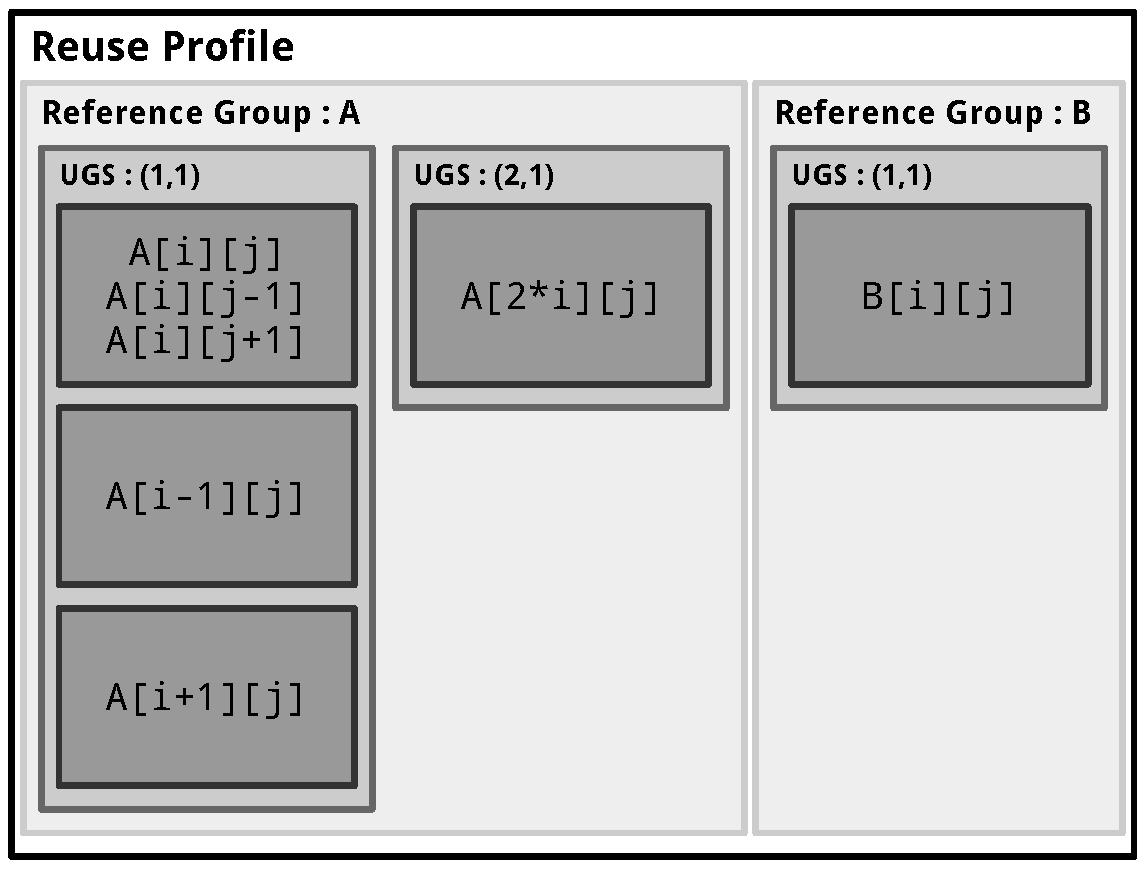
\includegraphics[width=\columnwidth]{images/Reuse_Profile_example1.pdf}
        \end{figure}
    \subsection{Parallelism}
        We say that a statement can be parallelized for a certain loop when it is legal to
        execute some different \textit{instances} of the statement (so with different iterators)
        on multiple cores at the same time, without violating any dependencies. The
        goal (not always possible) of executing multiple instances at the same time is to
        speed up the overall execution of the program.

        Unlike \textit{Data Reuse} where we had to find a good way to detect and characterize it,
        the \textit{Parallelism} of a statement doesn't need to be "characterize" :
        a statement can either be parallelized for a certain loop or it cannot : no more, no less.

        So in the end, the \textit{Parallelism Profile} of a statement is just the list
        of loop that can be parallelized safely for this statement.
        And to determine which loop can be parallelized safely, we just need to analyze
        the \glspl{self-dependence} of the statement. We only analyze \gls{self-dependence}
        because we analyze the statement alone, without any of the other statement of
        the scop, so the only possible dependencies are the one from the statement to itself.
        Dependencies in the polyhedral model are explained in the Section~\ref{sec:dependence_relations}.
       
        \bigskip

        Because we analyze the \glspl{self-dependence} of a statement, the only
        dependence we will find to analyze are Read-after-Write or Write-after-Read dependencies :
        \begin{itemize}
            \item Read-after-Read dependencies doesn't prevent parallelization because there is no
                change made to the memory location in question, so we don't even look at them.
        
            \item Write-after-Write dependencies don't concern us here because there is
                only one \textit{write} to the memory per statement which means that
                the \textit{source} and \textit{target} statement of Write-after-Write
                dependencies are always different, which is not out case here.
        \end{itemize}
        
        So once we've computed all the dependencies possible (for all the depth $d$ possible),
        we need, for all the iterators/loops of the statement, to check if one of the dependencies
        is loop-carried :
        \begin{itemize}
            \item A statement can be parallelized for a certain loop if none of its \glspl{self-dependence}
                are loop-carried.
            \item On the contrary if any \gls{self-dependence} of a statement is loop-carried for an certain loop,
                the statement cannot be parallelized for this loop.
        \end{itemize}
        Moreover, if a statement doesn't have \textit{any} dependence, it means that the
        statement can be parallelized for all its loops.

        \bigskip

        To determine if a \textit{Dependence Relation} is loop-carried or not for a certain
        loop $l$, we just have to add to the linear system represented by the
        \textit{Dependence Matrix} the following constraints :
        \begin{itemize}
            \item A equality constraint between each of the $(l-1)$ first iterators
                of the \textit{source} and \textit{target} statements.
            \item A \underline{strict} inequality between the $l^{\text{th}}$ iterator of
                the \textit{source} and \textit{target} statements.
        \end{itemize}
        These additional constraints have the following meaning : if a dependence
        still exists between instances of the \textit{source} and \textit{target}
        statement in the $l^\text{th}$ iteration dimension
        \begin{itemize}
            \item even when all of their \textit{other} iterators are equal (the "equal" constraints),
            \item even when the \textit{source instance} and \textit{target instance} of the dependencies
                in the $l^\text{th}$ must be strictly different (the "strict inequality" constraint),
        \end{itemize}
        then the dependence is loop-carried for the loop $l$.

        Once the constraints have been added to the system, we just have to give it to a
        solver like PIP : if there is a solution, the dependence is loop-carried for $l$,
        else it is not.
        
    \subsection{Vectorization}
        \subsubsection{Principles}
        Vectorization is a special case of Parallelization where we try to unroll a loop a
        little and transform the scalar operations, that compute only one single pair of
        operand, to vector operations (SIMD operation : Single Instruction, Multiple Data),
        that compute multiple pair of operand at a time, so that the loop can run a little
        faster and more efficiently.

        One of the conditions for a statement to be vectorized is that the memory accesses
        that appear in it should have the same alignment in memory : the address of all the
        accesses modulo the size of vector registers should be the same for all the accesses
        of the statement.
        But techniques exist to transform non-aligned accesses to aligned accesses, like
        in this paper~\cite{Eichenberger:2004:VSA:996893.996853}, so we chose to ignore this
        condition, by considering that compilers are now capable of handling this problem.

        Because Vectorization is a special case of Parallelization, the way to detect it
        is a lot like the way to detect parallelization : it involves the analysis of
        the \glspl{self-dependence} of a statement. But unlike Parallelization, here we are
        only interested in a certain number of loops. Those loops are the ones whose iterators
        are used either in :
        \begin{itemize}
            \item the last dimension of the accesses of the statements when in row-major,
            \item the first dimension of the accesses of the statements when in column-major.
        \end{itemize}
        These loops also need to have a unit stride (increment of 1).

        We will call the loops validating these 2 conditions \textbf{candidate loops}.
        The other loops, the ones that don't validate the 2 conditions, are ignored for
        the rest of the analysis (even though they could have been parallel). This is
        because when we vectorize a statement, the accesses of consecutive instances have
        to access consecutive memory location which can only be the case when the iterator
        of the loop is used in the dimension were data reuse can occur and when it have a unit stride.
        To have a real unit stride, these loop also need to be the innermost loop of the loop nest
        surrounding the statement.
        
        But we consider that it is not necessary for a loop to be the innermost to be
        in the \textit{Vectorization Profile}, because to be in the profile
        we only want to know which loop \textbf{could} allow vectorization
        for the statement \textbf{if} this loop was the innermost. The loop may not be
        the innermost at the moment, but the \textit{Vectorization Profile} would tell
        us that if we find a way to make it the innermost, then we would unlock vectorization
        for this statement and for this loop.

        \bigskip

        We then need to analyze the \glspl{self-dependence} of the statement :
        \begin{itemize}
            \item If there is no dependence at all, then we can add all the 
                \textit{candidate loops} to the \textit{Vectorization Profile}.
            \item If there are dependencies, we only look at the dependencies that
                are carried by one or more of the \textit{candidate loops}.\\
                For all the remaining dependencies $D$ carried by the loop $l$,
                if $D$ is a Write-after-Write or Read-after-Write dependence, then $l$
                is removed from the \textit{candidate loops}.
                The other kinds of dependence are Write-after-Read Read-after-Read 
                which don't cause any problems for the vectorization, so we can ignore
                those kinds of dependencies.
        \end{itemize}
        The \textit{candidate loops} that are left are then added to the profile because they
        don't cause any threats to the vectorization.

        \bigskip

        The \textit{Vectorization Profile} in the end is end just the list of loops that
        \textbf{if} they are/become the innermost loop, we can then vectorize the statement.

        \subsubsection{Limitations}
        For the \textit{Vectorization Profile}, we have chosen to only analyse the statements
        as if they were the only statement of the loop nest : that's why we only talk
        about dependencies that are from and to the statement.

        This approach simplifies the problem, but adds a limitation to the profile :
        a statement could be vectorized if it is considered "alone" but can in fact not
        be vectorized because it has some dependencies with some other statements of the loop
        nest.

        For example, in the following code :
\begin{lstlisting}[frame=single, language=C, caption={Vectorization Profile limitation example}, label={lst:vectorization_limitation}]
for(i=1 ; i<N ; i++) {
    A[i-1]=B[i]+1; // S1
    C[i]=A[i]*2; // S2
}
\end{lstlisting}
    S1 doesn't have any \gls{self-dependence}, so the $i$ loop would be in its
    profile. But there is a Write-after-Read dependence between S1 and S2 : this dependence
    make the vectorization of S1 illegal.

    So if the \textit{Vectorization Profile} is used during an optimization vectorizing
    some statement, we still need to keep checking for inter-statement dependencies.

    %XXX if the size of the vector register is smaller than minimum of all the access
    %A[i-offset], then we can still vectorize, but it's a borderline case.

    \subsection{Tiling Hyperplane}
        %TODO explain Hyperplane
        A Tiling Hyperplane is an hyperplane according to which we could tile a loop nest.
        
        There is generally a lot of Tiling Hyperplanes possible for a loop nest, and the difficulty
        is to find the optimal one.

        The paper~\cite{Bondhugula:2008:PAP:1379022.1375595}, described in the section~\ref{sec:auto_poly_paral}
        describes an algorithm that should compute the best Tiling Hyperplane for automatic
        parallelization and locality optimization.

        This algorithm is implemented in a program called \textbf{Pluto}~\cite{pluto} (which also
        uses the polyhedral model) and its results are really impressive.

        Because of that, we had the idea to use the Tiling Hyperplane computed by \textit{Pluto}
        as a property of a statement : after all, the Tiling Hyperplane computed is
        \textit{Pluto}'s way of seeing the statement.

        The Tiling Hyperplane Profile of a statement would simply be composed
        of the Tiling Hyperplane vectors/matrix \textit{Pluto} has computed for
        it when it is alone : meaning that we remove every other
        statement of the scop so that Pluto computes the Tiling Hyperplane for this \textit{specific}
        statement).

        %\bigskip

        %But the way we see the Tiling Hyperplane Profile is a little different from the way we see
        %the other profile types. Every other profile types can be used alone to aggregate
        %statements solely based on them, but the way we see the Tiling Hyperplane Profile is
        %that it needs to be used in partnership with other profile types, but not alone.
        %Because using it alone would 
    %\subsection{Register Pressure}

\section{SuBStrAte : Aggregating "Near Behaving" Statements Using Profiling}
    Substrate is the result and the implementation of the work and the research I've done
    on how to profile the different properties of a statement and how to aggregate similar
    statements.\\
    Substrate is a program that will profile each statement of a \textit{scop} for
    each each of its properties with the analysis pass.

    It will then try to aggregate
    statements into what I call \textbf{meta-statement}. Meta-statements are simply
    aggregated statements seen as one statement (in the way the polyhedral see statements)
    : it has the same \textit{Domain} and \textit{Scattering} than all its statements,
    all the memory accesses of all the statements are the memory accesses of the \textit{meta-statement}.

    To aggregate statements into meta-statements, we need to rate the similarity between two
    statements (or meta-statements) : putting a numerical value to their similarity.
    If the similarity is high, the rate is high, and if the rate is high, we need to
    aggregate the statements.

    So I had to find a way to rate this similarity : transforming the comparison between
    2 profile into a numerical value.

    \subsection{Statement Profiling}
    The analysis pass is the direct implementation of \textit{Profile Type} model explained in section~\ref{sec:statement_profiling}:
    \begin{itemize}
        \item The Reuse Profile is built by grouping the
            different memory accesses into array reference groups, then uniformly generated set groups,
            then groups with the same reuse direction. The harder part here wasn't the
            implementation but the research.

        \item The Parallelism Profile is built by listing all the loop indexes that could be
            parallelized for the statement. It is done by using the loop carried algorithm
            of the polyhedral model : if for a loop index, not a single one dependence is
            loop carried by it, then it can be safely parallelized.
            The catch in our case was that the implementation of this algorithm was in
            \textbf{CAnDL}, another library/program of the \textit{periscop} suite (a suite of
            library/program using the OpenScop format). \textit{CAnDL} can compute
            a lot of things regarding the \textit{dependence} in the \textit{polyhedral model},
            but its implementation of the loop carried algorithm wasn't working due to old
            changes in \textit{OpenScop} specification that were never correctly/fully implemented
            for this function/algorithm.
            
            So I had to fix the implementation without breaking anything.
            Some parts of the code weren't making any sense, slowing me down because I had
            to figure out what I could safely remove, what I couldn't remove, and what I
            had to fix.

            In the end, the function is now working, and as a side effect of the time I've taken
            to fix it, I've added to \textit{CAnDL} a function that computes if a dependence
            is loop independent or not.
        \item The Vectorization Profile building algorithm
            , like I explained in the section~\ref{sec:statement_profiling}, is a lot like
            the Parallelism profile building algorithm, but with some additional checks.
            In the end, the Vectorization profile is simply the list of loop indexes for which
            the statement \textit{could be} vectorized if they were the innermost loop of the loop nest.\\

            And because the fix of the loop carried function of \textit{CAnDL} was done during
            the implementation of the Parallelism profile, the implementation of the
            Vectorization profile took less time than planned.
        \item The Tiling Hyperplane Profile is not done by \textit{Substrate} but by
            \textbf{Pluto}~\cite{pluto} : \textit{Substrate} merely uses the results of
            \textit{Pluto}'s analysis to get the direction vector of the best Tiling Hyperplane
            \textit{Pluto} could find.

            But adding \textit{Pluto} to the project proved to be more difficult than expected.
            \textit{Pluto} builds all its dependencies itself, but I wanted to avoid that and
            to have Pluto use my versions of these dependencies, but I didn't want to tamper
            to much with its building process. Also, for \textit{Substrate} I've chosen \textbf{cmake}
            as the building system, and \textit{cmake} proved to be difficult to deal with in these
            sort of case.

            In the end, I gave in because I was losing too much time, and I let \textit{Pluto} build
            its own dependencies, even if it meant a lot of useless compilations.
    \end{itemize}
    
    \subsection{Similarity rating algorithms}
    To aggregate 2 statements or meta-statements, they need to be similar enough. We characterize
    this similarity, we propose the following approach :
    \begin{itemize}
        \item We rate the similarity between 0.0 and 1.0 for each of the 2 statements' profile types
            (the rating algorithms are described later).
        \item We use those rates to compute a weighted average.
        \item We compare the result of the weighted average to the minimal rates necessary
            to aggregate and if it is greater or equal to it, we aggregate the statements.
    \end{itemize}
    So the user has to give to the program the weight of each profile type as well as the
    minimal value the weighted average rate needs to be to aggregate.


    I choose to go with the weighted average rate because it allows us and the users
    to have a large control over the way \textit{substrate} handles the aggregation.
    Another reason was that with the proliferation of profile types, we didn't have
    any concrete idea to automatically weight the different profile types, so I decide
    to simply give manual control over it.
        \subsubsection{Data Reuse}
            Just a quick reminder, the Reuse Profile is built as the following : for all memory accesses of
            a statement, we first group them by reference, then by Uniformly Generated Set,
            then by reuse direction. The Reuse Profile Rating Algorithm simply counts
            the number of accesses of a statement that would belong to the same reuse
            direction group (so also the same reference group and Uniformly Generated Set group)
            of the other rated statement.
            
            In other words, the algorithm counts the accesses in direction group that match
            the same group in the other statement. If a statement has a direction group that doesn't
            have any matching group with the other statement, then the number of accesses contained
            in this group are not counted.

            We then take this counter and divided it by the total number of accesses of
            the 2 statements.

            For example :
\begin{lstlisting}[frame=single, language=C, caption={Reuse profile rating example}, label={lst:rp_example}]
for(i=0 ; i<N ; i++)
    for(j=0 ; j<N ; j++)
    {
        A[i][j] = A[i][j+1] + A[i+1][j] + B[i] + B[2*i];    //S1
        C[i][j] = A[i][j+2];                                //S2
    }
\end{lstlisting}
        In this example, S1 would have the following Reuse Profile :
\begin{figure}[H]
    \center
    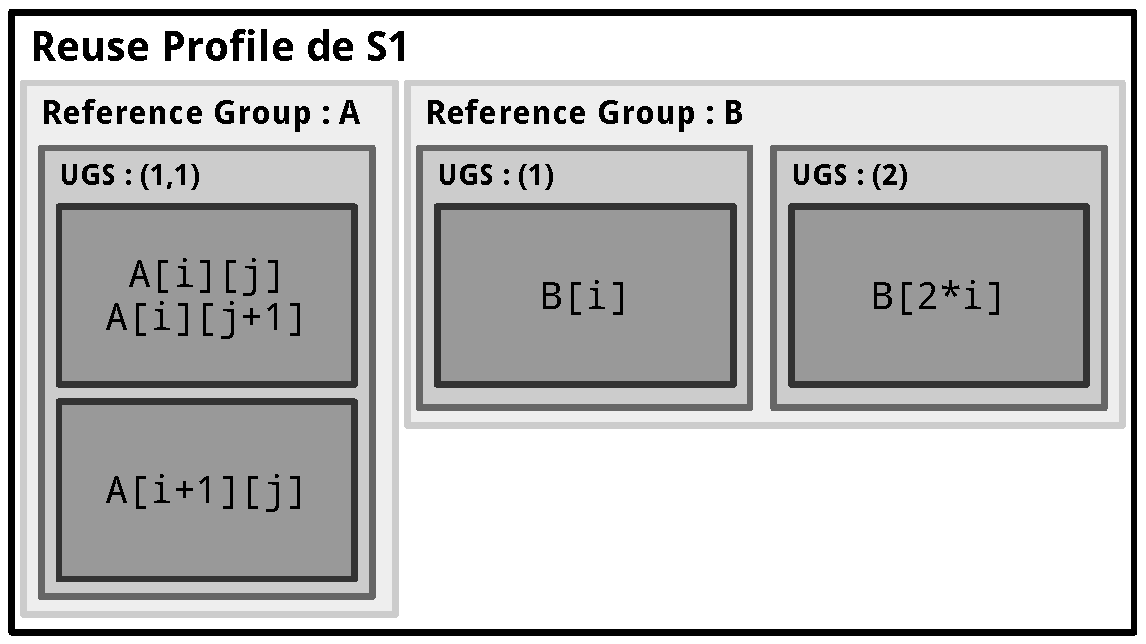
\includegraphics[width=\columnwidth]{images/Reuse_Profile_example2.pdf}
    \caption{Graphical represention of the Reuse Profile of S1}
\end{figure}
            and S2 would have the Reuse Profile :
\begin{figure}[H]
    \center
    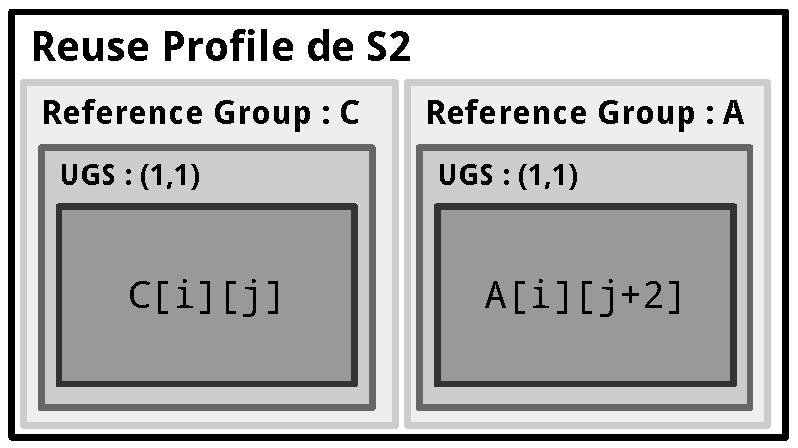
\includegraphics[width=0.7\columnwidth]{images/Reuse_Profile_example3.pdf}
    \caption{Graphical represention of the Reuse Profile of S2}
\end{figure}
        we can see that the group ${A[i][j],A[i][j+1]}$ of S1 matches the group ${A[i][j+2]}$
        of S2 : so we count $3$. There is no other match between the groups of the 2 statements,
        so the final value of the counter is $3$. The total number accesses is $7$, so the
        Reuse Rate between the two statement is :
        \begin{center}
            $\dfrac{\mathit{Counter}}{\mathit{Total\_number\_accesses}} = \dfrac{3}{7} \approx 0.43$
        \end{center}

        \bigskip

        You can see that even though S2 just have one access in common with S1, we still get
        a "relatively" high rate : this is because S1 has the lot of reuse for a particular
        direction group, and S2 has an access that match that group.

        With a rate of $0.43$, it means that $43\%$ of the memory accesses made by the 2 statements accesses
        read/write the same memory area, with the same direction. Which means that if the
        CPU cache is big enough, $43\%$ of the memory accesses lead to \textbf{cache hits}.
            
        \subsubsection{Parallelism}
            Because the Parallelism Profile of a statement is simply the list of loops
            which could be legally parallelized for the statement, we chose to count the
            loops in common that could be parallelized for both statements, and then
            divide that by the total number of loops that could be parallelized for either
            of the statements :
            \begin{center}
                $ \mathrm{Parallelism\_Rate} =  \dfrac{\mathrm{Card}( {PP_1} \cap {PP_2})}{\mathrm{Card}({PP_1} \cup {PP_2})}$
            \end{center}
            with $PP_1$ being the parallelism profile of the first statement, and $PP_2$ 
            the second statements'.

            \bigskip

            For example :
\begin{lstlisting}[frame=single, language=C, caption={Parallelism profile rating example}, label={lst:pp_example}]
for(i=0 ; i<N ; i++)
    for(j=0 ; j<N ; j++)
        for(k=0 ; k<N ; k++)
            for(l=0 ; l<N ; l++)
            {
                S1(i,j,k,l);
                S2(i,j,k,l);
            }
\end{lstlisting}
        Let say the parallelism profile of S1 and S2 are respectively $\{i,j\}$ and $\{j,k\}$.
        The parallelism rate between those 2 statements would be :
        \begin{center}
            $\dfrac{\mathrm{Card}( \{i,j\} \cap \{j,k\})}{\mathrm{Card}( \{i,j\} \cup \{j,k\})}
            = \dfrac{\mathrm{Card}( \{i\})}{\mathrm{Card}( \{i,j,k\})}
            = \dfrac{1}{3}
            = 0.333...$
        \end{center}

        \subsubsection{Vectorization}
            Because the Vectorization Profile is, like the Parallelism Profile, 
            simply a list of loops, the rating algorithm for the Vectorization Profile
            is the same as the one for the Parallelism Profiles :
            \begin{center}
                $ \mathrm{Vectorization\_Rate} =  \dfrac{\mathrm{Card}( {VP_1} \cap {VP_2})}{\mathrm{Card}({VP_1} \cup {VP_2})}$
            \end{center}
            with $VP_1$ and $VP_2$ the Vectorization Profile of respectively the first and second rated statements.
        \subsubsection{Tiling Hyperplane}
            Because the Tiling Hyperplane Profile is simply the list of vectors
            Pluto has computed for the Hyperplane, we've decided to compute the strict
            equality for the rating algorithm : 
            \begin{center}
                $ \mathrm{Tiling\_Hyperplane\_Rate} =  \left \{
                    \begin{array}{c}
                        0.0\text{, if } \mathit{THP}_1 \neq \mathit{THP}_2. \\
                        1.0\text{, if } \mathit{THP}_1 = \mathit{THP}_2.
                    \end{array} \right.$
            \end{center}
            with $\mathit{THP}_1$ and $\mathit{THP}_2$ the Tiling Hyperplane Profile of 
            respectively the first and second rated statement.

            We are aware that this rating algorithm doesn't allow to precise control using the
            Tiling Hyperplane Profile, because of the "All or Nothing" approach,
            but this profile type was the last implemented, and its rating
            algorithm hasn't mature enough yet.
        %\subsubsection{Register Pressure}

    \subsection{Statement Profile Aggregation}
        When we aggregate 2 statements, we also aggregate their different profiles together.
        Here are the different profile aggregation algorithms.
        \subsubsection{Data Reuse}
            In the case of the Data Reuse Profile, we recursively aggregate the Reuse Profiles :
            \begin{itemize}
                \item First we try to compare the Reference groups of the 2 Reuse Profiles :
                    if for the Reference group of a profile there is a Reference group in
                    the other profile that has accesses to the same array reference, then
                    we recursively aggregate these 2 Reference groups. If there is no
                    match, then we just add the Reference group to the new Reuse Profile.
                \item We then do the same for the Uniformly Generated Set groups of the
                    Reference groups we are trying to recursively aggregate. Which means we
                    try to find 2 matching Uniformly Generated Set groups.
                    If that's the case, we try to recursively aggregate them, if not we simply
                    add them to the current Reference group of the new Reuse Profile.
                \item And finally we do the same for the Direction group.
            \end{itemize}
            
            Or in other word, we just fuse matching Direction groups,
            and add the rest non-matching groups without touching them.
        \subsubsection{Parallelism}
            In the case of the Parallelism Profile, we compute the intersection between
            the list of loops from the first and second Parallelism Profile. The result
            of the intersection is the Parallelism Profile of the newly aggregated statement.
        \subsubsection{Vectorization}
            Because the Vectorization Profile is very similar to the Parallelism Profile, 
            the Profile Aggregation Algorithm is the same : the intersection between the
            list of loops from the first and second Vectorization Profile, with the result
            being the Vectorization Profile of the newly aggregated statement.
        \subsubsection{Tiling Hyperplane}
            In the case of the Tiling Hyperplane Profile, because it is so tied to how
            Pluto works, and because Pluto can possibly compute a different Tiling Hyperplane
            of an aggregated statement from the ones it computed when the statements weren't
            aggregated, we decide to let Pluto re-compute the Tiling Hyperplane for the newly
            aggregated statement : we simply delegate it to Pluto.
        %\subsubsection{Register Pressure}
        \subsubsection{Polyhedral Representation}
            We also need to aggregate the Polyhedral Representation of the 2 statements.
            Because the 2 statements need to have the same \textit{Domain Relation}, should be
            successive and have the same loop depth, then the aggregated statement will have
            the same \textit{Domain Relation} and \textit{Scattering Relation} than the first
            statement. For the \textit{Access Relations} of the result statement, we
            are computing the union of \textit{Access Relations} of the 2 aggregated statements :
            if there are duplicate \textit{Access Relations}, we only keep one copy.
            By doing so, we decrease the overall number of dependencies between statements,
            thus decreasing the complexity of the representation.
            

    \subsection{Statement Aggregation Strategy}
        Now that we have defined how we rate the similarity between the profiles of 2 statement,
        it is possible to use the similarity rate to aggregate or not 2 statements, but
        we still need to define an aggregation strategy : should we start from the first
        statement, the last or the one in the middle ? Should we aggregate in that order
        or this order ? Should we introduce some randomness ?

        In the end, we did not have enough time to implement more than one strategy. We
        have some ideas for additional strategies, and they are described in the section
        \ref{sec:future_works}. We will present here the only strategy that is currently implemented
        in \textit{Substrate}.
        \subsubsection{Successive Statements Aggregation}
            The Successive Statements Aggregation Algorithm (SSAA) iterate through
            the statements of a scop, from the first statement of the scop to the last.
            For each statement S1, it looks at the next statement S2 in the scop, and
            checks if :
            \begin{itemize}
                \item S1 and S2 share the same Domain Matrix.
                \item S1 and S2 share the same Scattering Matrix, and the same beta depth
                    (i.e. they are in the same loop nest and have the same depth in that nest).
            \end{itemize}
            If these conditions are met, SSAA then rates the similarity between S1 and S2,
            and if the rate is greater or equal to the minimal rate the user gave to \textit{Substrate}
            then it aggregates S1 and S2 into S3. S3 then takes the place of S1, and everything starts
            over.

            If the conditions are not met, then S2 takes the place of S1 and everything starts over.
            

\section{Experiments and Results}
In this section, we will discuss the experiments we've conducted and the consequences
of their results.
We need to keep in mind in this section that currently, only the aggregation strategy 
"Successive Statement Aggregation Algorithm" (SSAA) is implemented and used by \textit{Substrate}.
So when we say than \textit{Substrate} is aggregating statements, it is implied that it uses
the SSAA.

\bigskip

From the beginning, we wanted to beat \textit{Pluto}, which is consider as
one of, if not \textbf{the}, best optimizer available today.\\
Of course, it is impossible for us, at least for now, to go completely without using \textit{Pluto}:
we still use \textit{Pluto} to optimize, but it now takes its input from us, and does
not come first.

What we do is that we give \textit{Pluto} the scop we have optimized with \textit{Substrate}.
We then take the optimized code it produces from our optimized scop,
and compare its performance with the optimzed code \textit{Pluto} would have produce from
the original code, without our help.

We proceed this way because we noticed that in some case, \textit{Pluto} wasn't able
to find the best optimization possible, sometimes even producing optimized code that would
perform worse than the original, non optimized, code. So we wanted to see if we could
guide \textit{Pluto}, so that it can find the best optimization possible.

But first, we need to discuss about the program we used for our experiments. With the subject
of this internship was given a concrete example of a code that we knew Pluto was not able to optimize correctly.
The original code is the following :
\begin{lstlisting}[frame=single, language=C, caption={Origin Conventional Beamforming kernel}, label={lst:original_conventional_beamforming}]
for (i = 0; i < N; i++) {   //L1
  a_i[i] = 0;                                           //S1
  a_r[i] = 0;                                           //S2
  for (j = 0; j < M; j++) { //L2
    a_r[i] += s_r[j] * m_r[i][j] - s_i[j] * m_i[i][j];  //S3
    a_i[i] += s_i[j] * m_r[i][j] + s_r[j] * m_i[i][j];  //S4
  }
  val = a_r[i] * a_r[i] + a_i[i] * a_i[i];              //S5
  t = (val >= t_val)? (t_val = val, i) : t;             //S6
}
\end{lstlisting}
we can that S3 and S4 share a lot of data reuse. But if we give this code to \textit{Pluto},
it will separate S3 and S4 in 2 different parallel loops, loosing the data locality, as you
can see in Listing~\ref{lst:pluto_conventional_beamforming} :
\begin{minipage}[t]{0.45\textwidth}
\begin{lstlisting}[frame=single, language=C, basicstyle=\scriptsize, caption={Conventional Beamforming kernel optimized by Pluto}, label={lst:pluto_conventional_beamforming}]
#pragma omp parallel for
for (i = 0; i <= N - 1; i++)
  a_r[i] = 0;

#pragma omp parallel for
for (i = 0; i <= N - 1; i++)
  for (j = 0; j <= M-1; j++)
    a_r[i] += s_r[j] * m_r[i][j]
      - s_i[j] * m_i[i][j];

#pragma omp parallel for
for (i = 0; i <= N - 1; i++)
  a_i[i] = 0;

#pragma omp parallel for
for (i = 0; i <= N - 1; i++)
  for (j = 0; j <= M - 1; j++)
    a_i[i] += s_i[j] * m_r[i][j]
      + s_r[j] * m_i[i][j];

for (i = 0; i <= N - 1; i++) {
  val = a_r[i] * a_r[i] + a_i[i] * a_i[i];
  t = (val >= t_val)? (t_val = val, i) : t;
}
\end{lstlisting}
\end{minipage}
\hfill
\begin{minipage}[t]{0.45\textwidth}
\begin{lstlisting}[frame=single, language=C, basicstyle=\scriptsize, caption={Goal version of Conventional Beamforming kernel}, label={lst:substrate_conventional_beamforming}]
#pragma omp parallel for
for (i = 0; i <= N - 1; i++) {
  a_r[i] = 0;
  a_i[i] = 0;
  for (j = 0; j <= M - 1; j++) {
    a_r[i] += s_r[j] * m_r[i][j]
      - s_i[j] * m_i[i][j];
    a_i[i] += s_i[j] * m_r[i][j]
      + s_r[j] * m_i[i][j];
  }
}

for (i = 0; i <= N - 1; i++) {
  val = a_r[i] * a_r[i] + a_i[i] * a_i[i];
  t = (val >= t_val)? (t_val = val, i) : t;
}
\end{lstlisting}
\end{minipage}
But as you can see in Listing~\ref{lst:substrate_conventional_beamforming}, the best optimization
would be to let S3 and S4 together in a parallel loop, thus exploiting the data locality
shared by them.

\bigskip

All of this explains why Listing~\ref{lst:original_conventional_beamforming} became one
of the program of our benchmark suit. But we needed more programs, and those programs needed to
fit the polyhedral model, so decided to use the ones provided by the \textbf{PolyBench},
the Polyhedral Benchmark suite, which contains a lot of different codes, all of them fitting
the polyhedral model. It was also the occasion to try and see how many programs of the \textit{PolyBench}
were affected by \textit{Substrate} : if it was even possible to aggregate some of their statements.

What we found was that only 7 programs out of the 30 of the \textit{PolyBench} are eligible
 for our benchmark suit : bicg.c , correlation.c, covariance.c, deriche.c, durbin.c, gesummv.c, symm.c.
The other programs of \textit{PolyBench} were not eligible because none of their statements could be
aggregated by \textit{Substrate}, even when run with the lowest minimum aggregation rate possible : 0.0.
The reasons for that are that these programs are either too short, each of their
successive statements have different \textit{Domain Matrix} or they have no similarity at all.
All of these reasons resulting in zero aggregation. It is however important to remark that
this number could possibly change with an aggregation strategy different from SSAA.

\bigskip

In the end, our benchmark suit is comprised of the 7 selected programs of the \textit{PolyBench}
and the Conventional Beamforming kernel (Listing~\ref{lst:original_conventional_beamforming}).

\subsection{Number of statement aggregated per Profile Type}
\label{sec:nb_stmt}

Even though \textit{Substrate} can do multi-criteria aggregation, we wanted to see first what
the results would be for simple mono-criteria aggregations.\\
We first wrote a script running \textit{Substrate} on our benchmark suit, forcing it to
only aggregate statements according to one Profile Type, for each Profile Type implemented
and minimal aggregation rate ranging from 0.0 to 1.0.\\

We were interested to see how many statement were aggregated per Profile Type and per minimal
aggregation rate. The results are shown in the next pages.

We can already notice that bicg.c and symm.c (Figure~\ref{fig:nb_stmts:bicg}|\ref{fig:nb_stmts:symm})
don't show a lot of similarity : just some reuse for low aggregation rate, but that's all.
The same can be said for durbin.c (Figure~\ref{fig:nb_stmts:durbin}) : the only profile type
inducing aggregation is Tiling Hyperplane, but as we said before this Profile Type should not
be used alone.
What it means is that \textit{Substrate} is not really useful for these programs. Even though
it can aggregate some statements, their similarity is too low to be useful. On the contrary
it could be harmful because it could prevent good optimization from happening.

gesummv.c seems promising because it shows enough similarity for aggregation even at high
minimal aggregation rate. Only data reuse is left behind, with statements aggregation only
for low minimal aggregation rate.

The next 3 programs (conventional\_beamforming.c, correlation.c, covariance.c) show a lot of
similarity : there is aggregation even with high minimal aggregation rate ( 0.6), and
there is generally 3 Profile Type inducing these aggregations, meaning that those aggregated 
statements share similarity for more than one or two of their properties.

And finally there is deriche.c (Figure~\ref{fig:nb_stmts:deriche}). deriche.c shows good
Data Reuse and Tiling Hyperplane similarity.\\

To be clear, these results only show us how useful \textit{Substrate} could \textbf{potentially} be.
To be sure, we need to confront these result to the time we get for them during their optimization by Pluto
and during their execution.


%\newgeometry{
    %bottom=40mm}
\begin{figure}[H]
    \center
    \includegraphics[width=\linewidth]{results/nb_stmts/bicg.c.scop.results}
    \caption{bicg.c}\label{fig:nb_stmts:bicg}
    \includegraphics[width=\linewidth]{results/nb_stmts/symm.c.scop.results}
    \caption{symm.c}\label{fig:nb_stmts:symm}
\end{figure}
\begin{figure}[H]
    \center
    \includegraphics[width=\linewidth]{results/nb_stmts/durbin.c.scop.results}
    \caption{durbin.c}\label{fig:nb_stmts:durbin}
    \includegraphics[width=\linewidth]{results/nb_stmts/gesummv.c.scop.results}
    \caption{gesummv.c}\label{fig:nb_stmts:gesummv}
\end{figure}
\begin{figure}[H]
    \center
    \includegraphics[width=\linewidth]{results/nb_stmts/conventional_beamforming.c.scop.results}
    \caption{conventional\_beamforming.c}\label{fig:nb_stmts:conv_beam}
    \includegraphics[width=\linewidth]{results/nb_stmts/correlation.c.scop.results.png}
    \caption{correlation.c}\label{fig:nb_stmts:correlation}
\end{figure}
\begin{figure}[H]
    \center
    \includegraphics[width=\linewidth]{results/nb_stmts/covariance.c.scop.results}
    \caption{covariance.c}\label{fig:nb_stmts:covariance}
    \includegraphics[width=\linewidth]{results/nb_stmts/deriche.c.scop.results}
    \caption{deriche.c}\label{fig:nb_stmts:deriche}
\end{figure}
\restoregeometry

\subsection{Speedup of Pluto's runtime}
\label{sec:speedup_pluto}

We know that aggregating statements reduces the complexity of the polyhedral representation
of a program, because it means less statements and less dependencies (because in the case
of statements sharing identical memory accesses, the duplicate accesses are removed when aggregated).
But we wanted to see if a less complex polyhedral representation really leads to shorter
times of optimization, at least from \textit{Pluto}.

\bigskip

To test that, we wrote a script that calls \textit{Pluto} to optimize every optimized scop produced
by \textit{Substrate} in the section~\ref{sec:nb_stmt} (so per Profile Type and minimal aggregating rate),
and record the time it took. The script then does the same but this time with the scop of
the original source code of the program, so \textbf{not optimized} by \textit{Substrate}.\\
Every time \textit{Pluto} was called was with the option \verb'--parallel', and the benchmark
was run on a T9400 (Intel Core 2 Duo, 2.53GHz) with 2GB of DDR2.

\bigskip

We then compare the time it took for \textit{Pluto} to optimize with our optimized scop and
the original scop. The results can be found in the next pages.

To understand them, we need to compare each of them to their respective graph in the section~\ref{sec:nb_stmt}.
If we do that, we can see that almost every time statements are aggregated in a program,
there is a speedup of Pluto's runtime. The speedup is generally around 1.2 (bicg.c, symm.c, durbin.c, covariance.c),
but it can get higher like 1.5 for correlation.c and 1.9 for deriche.c . It seems like there
is a correlation between the number or percentage of aggregated statements in a program and
the speedup we get for \textit{Pluto}'s runtime : the greater the percentage of aggregation,
the greater the speedup.

\bigskip

These results are encouraging because they would mean that even if our optimization pass
may doesn't always induce better final code optimization, it still induces faster runtime
for optimizer.

\bigskip

Of course, we need to show that the time we lose when \textit{Substrate} optimizes a scop
doesn't outweigh the time we gain with \textit{Pluto}. This is not done yet, but we are planning
to do it before the end of the internship.


%\newgeometry{
    %bottom=40mm}
\begin{figure}[H]
    \center
    \includegraphics[width=\linewidth]{results/pluto/bicg.c.results}
    \caption{bicg.c}\label{fig:pluto:bicg}
    \includegraphics[width=\linewidth]{results/pluto/symm.c.results}
    \caption{symm.c}\label{fig:pluto:symm}
\end{figure}
\begin{figure}[H]
    \center
    \includegraphics[width=\linewidth]{results/pluto/durbin.c.results}
    \caption{durbin.c}\label{fig:pluto:durbin}
    \includegraphics[width=\linewidth]{results/pluto/gesummv.c.results}
    \caption{gesummv.c}\label{fig:pluto:gesummv}
\end{figure}
\begin{figure}[H]
    \center
    \includegraphics[width=\linewidth]{results/pluto/conventional_beamforming.c.results}
    \caption{conventional\_beamforming.c}\label{fig:pluto:conv_beam}
    \includegraphics[width=\linewidth]{results/pluto/correlation.c.results.png}
    \caption{correlation.c}\label{fig:pluto:correlation}
\end{figure}
\begin{figure}[H]
    \center
    \includegraphics[width=\linewidth]{results/pluto/covariance.c.results}
    \caption{covariance.c}\label{fig:pluto:covariance}
    \includegraphics[width=\linewidth]{results/pluto/deriche.c.results}
    \caption{deriche.c}\label{fig:pluto:deriche}
\end{figure}
\restoregeometry



\subsection{Speedup of the program runtime}

We wanted to know if what we were doing since the beginning had a real impact on the time they
take to run. To test that, we've wrote a script compiling and then running the optimized code
produced by \textit{Pluto} in the section~\ref{sec:speedup_pluto} from our optimized scop and
from the original scop. We then record the time it took for each of them and then compare
the runtime of the code produced by \textit{Pluto} from our optimized scop with the code
optimized by \textit{Pluto} alone, to see if we can get a speedup.\\
The code were compiled by gcc with the options \verb'-O3 -lm -fopenmp', and were run for
the benchmark on a Q6600 (Intel Quad, 2.40GHz, 8Mo L2) with 4GB DDR2 667Mhz.

The results can be found in the next pages. 

\bigskip

From the 8 programs of our benchmark suit, only conventional\_beamforming.c,
correlation.c and covariance.c show significant speedup with respectively an average speedup of
1.5, 1.7 and 1.65. The other programs of the benchmark show an average speedup of 1, meaning
that they don't run any slower of faster than the optimized code produced by \textit{Pluto} alone,
which indicates that even though we find similarity and aggregate accordingly to it, \textit{Pluto}
could have done it without us.

But these results also show that our optimization pass is really working, even if
it's on limited cases, and that when it works, the results are really encouraging.

%\newgeometry{
    %bottom=40mm}
\begin{figure}[H]
    \center
    \includegraphics[width=0.9\linewidth]{results/runtime/conventional_beamforming.c.results}
    \caption{conventional\_beamforming.c}\label{fig:runtime:conv_beam}
\end{figure}
\begin{figure}[H]
    \center
    \includegraphics[width=\linewidth]{results/runtime/correlation.c.results.png}
    \caption{correlation.c}\label{fig:runtime:correlation}
    \includegraphics[width=\linewidth]{results/runtime/covariance.c.results}
    \caption{covariance.c}\label{fig:runtime:covariance}
\end{figure}
\restoregeometry

%\begin{figure}[H]
    %\begin{minipage}{0.50\textwidth}
        %\includegraphics[height=\linewidth, angle=-90]{results/nb_stmts/bicg.c.scop.results}
        %\caption{bicg.c}\label{fig:nb_stmts:bicg}
    %\end{minipage}\hfill
    %\begin{minipage}{0.50\textwidth}
        %\includegraphics[height=\linewidth, angle=-90]{results/nb_stmts/conventional_beamforming.c.scop.results}
        %\caption{conventional\_beamforming.c}\label{fig:nb_stmts:conv_beam}
    %\end{minipage}
    %%\begin[0.32\textwidth]{minipage}
    %%\end{minipage}\hfill
%\end{figure}
%Graph nb stmt aggrégé

    
\section{Conclusions}
The goal of this internship was to study smart ways to aggregate several statements
together to achieve a better performance as well as a better scalability for polyhedral
compilation frameworks.

\bigskip

We've started with the idea that similar or \textit{near behaving} statements should be
aggregated (considered as one instead of two). So we had to come up with a way to characterize
the "similarity" between two statements. For that purpose, we've proposed a model where
each statement is associated with a list of profile built during the analysis pass.
Each profile corresponds to a different property a statement can have like \textit{Data Reuse},
\textit{Parallelism} etc...\\
These profiles are a way to quantify or at least measure those properties, and this quantification
allows us to compare the profiles of 2 statements, with numbers. By comparing the profiles
of 2 statements, we are able to compute the Similarity Rate between them, and with that we're
able to characterize the similarity between 2 statements.\\
We have successfully implemented in \textit{Substrate} the profiles and rating algorithms of :
\textit{Data Reuse}, \textit{Parallelism}, \textit{Vectorization}, \textit{Tiling Hyperplane}.

The next thing we needed to do was to find Aggregation Strategies. An Aggregation Strategy
determines the way we plan to rate the similarity and aggregate the statements in a scop : in what
order, with or without randomness, with or without human help etc...\\
For now, only one Aggregation Strategy is implemented in \textit{Substrate},
and it is "Successive Statements Aggregation Algorithm" (SSAA).
SSAA tries to aggregate only successive statements, from the first to the last
statement of the scop, and even though it is a relatively simple algorithm, the results we
are getting by using it are promising.\\
Even though we've seen that our approach is not always applicable, when it does
we have noticed good runtime speedups, and an overall speedup of the time taken by \textit{Pluto}
to optimize after us, when we were able to aggregate some statements. It indicates that our idea,
our optimization pass shows good potential and than we should pursue our research on it.

    \subsection{What this internship has brought to me}
        I'm happy to say that I have learn a lot of and about new things during this internship :
        the polyhedral model, Data Reuse and Locality, Parallelism and Vectorization detection
        in the polyhedral model, Tiling Hyperplane, and some other.\\
        To do that, I had to to read, understand and summarize scientific papers which made
        me a little bit used to it.
        One of my goals was to learn and discover new things about compilation and optimization,
        and this goal is clearly achieved for me.

        I also wanted to know if I had what it takes to work in the Research and if I wanted
        to try to do a PhD thesis about compilation and optimization. This internship gave me
        the opportunities to answer some of my questions and even though some of them were
        not answered, I'm still glad to have learned things about myself.\\
        Without this internship, I think I would have never tried to apply for a PhD thesis.

        This internship was also the occasion to practice my programming skills. I didn't
        really learn anything new in C and Python programming, but it felt really nice to
        program in C again, and I had to contribute to some existing projects, and it was
        the first time I was the object of a code review : it was, I think, an important experience.

        An aspect of the internship I didn't expect to do was that I had to organize myself
        my time and my work : what I needed to do, when I should do it etc... It's not that I
        am not capable of being autonomous, it's just that I wasn't expecting to be
        \textbf{this} free. But I am autonomous by nature so I've quickly picked up the pace.

        And finally, there is one more thing I did not expect to do : practice my English skills.\\
        Because the ICPS team has a lot of foreigners, English is used a lot, and it has forced
        me to practice my English, to speak and understand people speaking with different accents.
        And of course I also had to practice my writing with this report.
        I am now more confident about my skills and I really less afraid to speak in English
        : I know more about my strengths and weaknesses in English, and I'm not that
        afraid anymore to speak in English.


\section{Future Works}
\label{sec:future_works}
At this point in the internship and for this subject, there are still many
questions to answer, problems to solve and many opportunities for improvement.
In this section, we want to mention which ideas we have for future works on \textit{Substrate},
what could be done before the end of the internship, and what would be conceivable with more time.
    \subsection{Additional Profiles Types}
        First, we would like to add more Profile Types to the Profile of the statements,
        like \textbf{Register Pressure}. It could be the key to better aggregations and would
        give us a more complete framework to work with for scop optimization.\\

        We are planning to implement the \textbf{Register Pressure} before the end of the
        internship, and to study if this property is significant enough to be used in the
        computation of the \textit{Similarity Rate}.
    \subsection{Additional Aggregation Strategies}
        There is only one Aggregation Strategy implemented in \textit{Substrate}, but
        there are still some things we could try :
        \begin{enumerate}
        \item[Successive Statements Aggregation with Greedy Algorithm]
            Instead of trying to aggregate the statements from the first to the last
            of the scop being optimized, maybe we should try to use a greedy algorithm
            to chose which successive statements of the scop should be aggregated first :
            the 2 successive statements showing the best Similarity Rate are aggregated
            first, then we pick the next 2 successive statements with the best Similarity Rate etc...
            until the Similarity Rate between all successive statements are below the minimum rate.\\
        \item[Statements Aggregation using Graphs with Greedy Algorithm]
            The \textit{Successive Statements Aggregation with Greedy Algorithm} only
            tries to aggregate successive statements, statements with the same domain,
            the same scattering and the same beta depth, but maybe we could try to
            use the Greedy Algorithm with the Similarity Rate between all statements,
            and try to move and relocate some statements (if the move is legal),
            making them successive, then aggregating them.
        \item[Statements Aggregation using Neural Network]
            We could try using a Neural Network or other Genetic Algorithms, instead
            of Greedy Algorithm, to chose which statements need to be aggregated to
            maximize the overall similarity of the scop.
    \end{enumerate}
    \subsection{Too much different Statement Separator Program}
        One of the goal of this internship was to find a way to aggregate statements
        of a scop to trigger better optimizations, or prevent bad optimizations or even
        reduce the complexity of some optimization.

        But in some cases, it could be beneficial to force 2 statements to be separated
        from each other, because together they prevent some optimization to be applied,
        or they interfere with each other.

        For example, take the following case :
\begin{lstlisting}[frame=single, language=C, caption={Statements Separation example}, label={lst:stmt_sep_example}]
for (i = 0; i < size; i++) {
    for (j = 0; j < size; j++) {
        sum += A[i][j]; //S1
        A[i][j] = 0.;   //S2
    }
}
\end{lstlisting}
        In this code, S2 could be fully parallelized if alone but not S1, and there is
        some reuse between S1 and S2.

        But if we separate S1 and S2 in 2 different loop nest and fully parallelize S2,
        the resulting code could be faster than the original one. Or maybe not, because
        we would have to trade some reuse for parallelism, and it could be slower.
        
        The question is left open, and that's why we would like to try and answer it, and it
        would be a good trail to follow during a possible PhD thesis.
    \textit{Dynamic Optimization}
        For now, the optimization is done statically and it necessitates the inputs of an
        user. Another approach could be to perform the optimization dynamically, at runtime,
        by collecting information during the execution of the program, and with them
        determining automatically which profiles are the most relevant for this scop, at
        this moment of the execution, etc...\\
        This question would also be a good starting point for a possible PhD thesis.

            
\printglossary

\bibliographystyle{plain}
\bibliography{biblio}
\end{document}
